\subsection{Black-Scholes Equation}
The Black-Scholes equation is a PDE that describes the depreciation in the price of a European call or put option at a given stock price and a given time.

\subsubsection{Definition}
\noindent
Let us define a European call or put option with the following assumptions:
\begin{itemize}
    \item Define \(\sigma\) to be the volatility of the underlying asset and \(r\) be the risk-free interest rate.
    \item The initial valuation of an option at a fixed stock price is  \(V(S,0) = f(t)\). Thus, the option at a given underlying stock price \(S\) and a given option expiry time \(t\) is \(V(S,t)\).
\end{itemize}

\noindent
Thus, the Black-Scholes equation is defined as follows \citep{Buchanan_black_scholes_2014}:
\begin{equation} \label{eq:black_scholes_equation}
    \frac{\partial V}{\partial t} + \frac{1}{2}\sigma^2 S^2 \frac{\partial^2 V}{\partial S^2} + rS\frac{\partial V}{\partial S} - rV = 0
\end{equation}

\subsubsection{Application of the Fourier Transform}
Let us take the Fourier Transform of \cref{eq:black_scholes_equation} with respect to \(S\). Thus, let \(\hat{V}(\kappa, t)\) be the Fourier Transform of \(V(S, t)\) with respect to \(S\).

\begin{equation}
    \mathcal{F}_S \left\{ \frac{\partial V}{\partial t} + \frac{1}{2}\sigma^2 S^2 \frac{\partial^2 V}{\partial S^2} + rS\frac{\partial V}{\partial S} -  rV \right\} = \mathcal{F}_S \left\{ 0 \right\}
\end{equation}

\noindent
Using \cref{fourier_linearity} and the fact that the integral of the zero function is zero,
\begin{equation}
    \mathcal{F}_S \left\{ \frac{\partial V}{\partial t} \right\} + \mathcal{F}_S \left\{ \frac{1}{2}\sigma^2 S^2 \frac{\partial^2 V}{\partial S^2} \right\} + \mathcal{F}_S \left\{ rS\frac{\partial V}{\partial S} \right\} - \mathcal{F}_S \left\{ rV \right\} = 0
\end{equation}

\noindent
Using \cref{fourier_scaling},
\begin{equation} 
    \mathcal{F}_S \left\{ \frac{\partial V}{\partial t} \right\} + \frac{1}{2}\sigma^2 \mathcal{F}_S \left\{ S^2 \frac{\partial^2 V}{\partial S^2} \right\} + r \mathcal{F}_S \left\{ S\frac{\partial V}{\partial S} \right\} - r \mathcal{F}_S \left\{ V \right\} = 0
\end{equation}

\noindent
Using \cref{fourier_derivative},
\begin{align}
    \mathcal{F}_S \left\{ \frac{\partial V}{\partial S} \right\} &= i \kappa \mathcal{F}_S \left\{ V(S, t) \right\} \\
    &= i \kappa \hat{V}(\kappa, t) \\
    \mathcal{F}_S \left\{ \frac{\partial^2 V}{\partial S^2} \right\} & = i \kappa \mathcal{F}_S \left\{ \frac{\partial V}{\partial S} \right\} \\
    & = -\kappa^2 \hat{V}(\kappa, t)
\end{align}

\noindent
Using \cref{fourier_multiplication},
\begin{align}
    \mathcal{F}_S \left\{ S\frac{\partial V}{\partial S} \right\} &= \frac{1}{2 \pi}( \mathcal{F}_S \left\{ S \right\} * \mathcal{F}_S \left\{ \frac{\partial V}{\partial S} \right\} ) \\
    &= \frac{1}{2 \pi}( \mathcal{F}_S \left\{ S \right\} * i \kappa \hat{V} ) \\
    \mathcal{F}_S \left\{ S^2 \frac{\partial^2 V}{\partial S^2} \right\} &= \frac{1}{2 \pi}( \mathcal{F}_S \left\{ S^2 \right\} * \mathcal{F}_S \left\{ \frac{\partial^2 V}{\partial S^2} \right\} ) \\
    &= \frac{1}{2 \pi}( \mathcal{F}_S \left\{ S^2 \right\} * -\kappa^2 \hat{V} ) \\
\end{align}

\noindent
Therefore,
\begin{align}
    \frac{\partial \hat{V}}{\partial t} + \frac{1}{2}\sigma^2 \mathcal{F}_S \left\{ S^2 \frac{\partial^2 V}{\partial S^2} \right\} + r \mathcal{F}_S \left\{ S\frac{\partial V}{\partial S} \right\} - r \hat{V} &= 0 \\
    \frac{\partial \hat{V}}{\partial t} + \frac{1}{2}\sigma^2 \frac{1}{2 \pi}( \mathcal{F}_S \left\{ S^2 \right\} * -\kappa^2 \hat{V} ) + r \frac{1}{2 \pi}( \mathcal{F}_S \left\{ S \right\} * i \kappa \hat{V} ) - r \hat{V} &= 0 \\
    \frac{\partial \hat{V}}{\partial t} - \frac{1}{4 \pi}\sigma^2 \kappa^2 ( \mathcal{F}_S \left\{ S^2 \right\} * \hat{V} ) + \frac{1}{2 \pi} r i \kappa ( \mathcal{F}_S \left\{ S \right\} * \hat{V} ) - r \hat{V} &= 0
\end{align}

\noindent
Thus,
\begin{equation}
    \label{eq:black_scholes_fourier}
    \frac{d \hat{V}}{dt} = \frac{1}{4 \pi}\sigma^2 \kappa^2 ( \mathcal{F}_S \left\{ S^2 \right\} * \hat{V} ) - \frac{1}{2 \pi} r i \kappa ( \mathcal{F}_S \left\{ S \right\} * \hat{V} ) + r \hat{V}
\end{equation}

\subsubsection{Initial and Boundary Conditions}
A simple linear function will be used as the initial option price for the ODE:
\begin{align}
    V(S_{max}, t)=0.15t + 148.5 \label{eq:black_scholes_equation_initial_condition}
\end{align}

\noindent
If the underlying stock of an option is worth nothing, then the option itself is worth nothing. This boundary condition can expressed as follows:
\begin{align}
    V(0, t) = 0
\end{align}

\noindent
Furthermore, since a call option is advantageous when the stock price \(S\) is greater than the exercise price \(E\) and a put option is only advantageous when the exercise price \(E\) is greater than the stock price \(S\), the following boundary conditions must be true.
\begin{align}
    V(S, t) = 
    \begin{cases}
        max(S-E, 0) & \text{if call option} \\
        max(E-S, 0) & \text{if put option}
    \end{cases}
\end{align}

\subsubsection{Numerical Solution to Black-Scholes Equation}
\cref{eq:black_scholes_equation} is a first-order ODE that can be easily numerically integrated. A numerical solution to \cref{eq:black_scholes_fourier} using a fifth-order Runge-Kutta approximation in Python is presented below. The Python code can be found in \cref{code:black_scholes_equation}.

\begin{figure}[H]
    \centering
    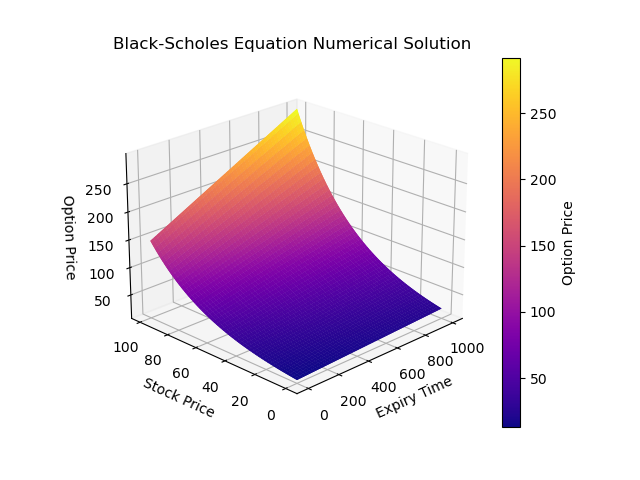
\includegraphics[width=100mm,height=\textheight,keepaspectratio]{images/black_scholes_equation_numerical.png}
    \caption{Defining the initial option price as \cref{eq:black_scholes_equation_initial_condition}, this plot shows the temperature change along \(S\) and \(t\) by performing a numerical integration of \cref{eq:black_scholes_fourier}.}
    \label{fig:black_scholes_equation_numerical}
\end{figure}